% https://tex.stackexchange.com/a/367681
\documentclass{beamer}
\usepackage{tikz}
\usetikzlibrary{positioning}
\begin{document}
\begin{frame}
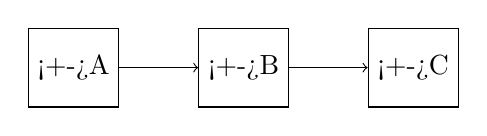
\begin{tikzpicture}[minimum size=1cm]
    \node<+->[draw,rectangle] (A) {\only<+->{A}};
    \node<+> (B) [right=of A] {};
    \node<+->[draw,rectangle] (B) [right=of A] {\only<+->{B}};
    \node<+> (C) [right=of B] {};
    \node<+->[draw,rectangle] (C) [right=of B] {\only<+->{C}};
    \draw<3->[->] (A.east) -- (B.west);
    \draw<6->[->] (B.east) -- (C.west); 
\end{tikzpicture}
\end{frame}
\end{document}
